\section{Design and Objectives}
\label{design}

To tackle this problem we run simulations of the CCD output for a given atom location using a raytracing simulation.  The output images are labeled according to atom location and used as a training set for machine learning algorithms.  The algorithms can then be used to generate a probabilistic distribution for the atom's location for a new CCD image.  

Figure \ref{fig:arch} describes the data flow of our architecture.  We begin by simulating the training and testing data using raytracing and filtering.  The filters will apply both generate several different training sets from a single image set.  The classification results for each training set are described below.  Some of the instances are selected from the image set for noise filtering.  The \emph{noisy} data is used to test our classification algorithms.

\begin{figure}[h]
\begin{center}
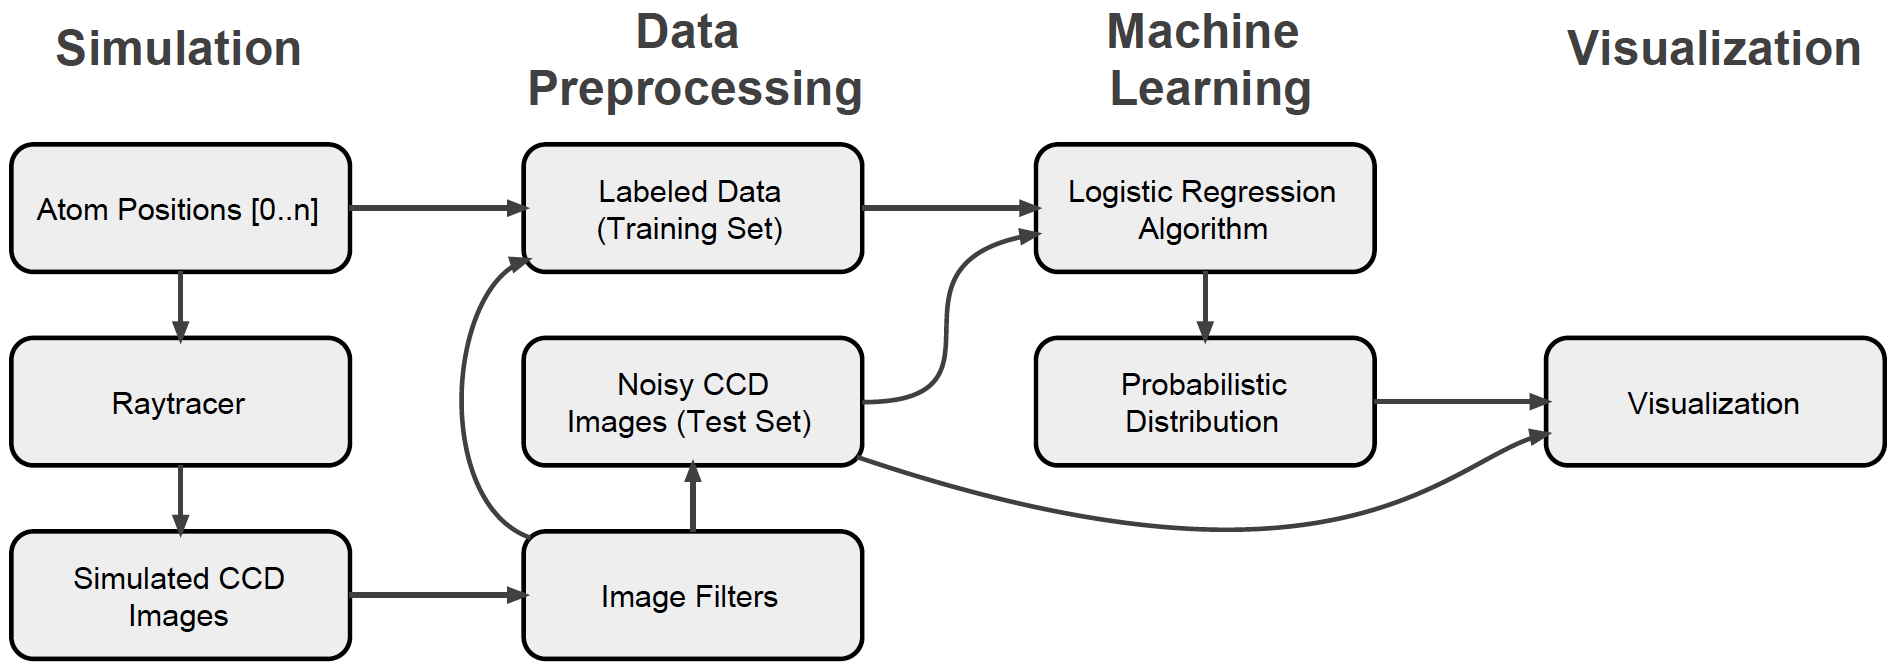
\includegraphics[scale=0.4]{arch.png}
\caption{High Level Data Flow Architecture Diagram}
\label{fig:arch}
\end{center}
\end{figure}

The objective of our project is to create and test a scalable machine learning solution for atom location prediction using CCD images.  In order to scale our application we use both shared memory and distributed memory parallelism.  Massive amounts of training data are generated using a shared memory parallelism, and a distributed memory logistic regression classifier is used to efficiently learn interesting patterns from the data.  The remainder of this report describes our development efforts, experimentation results, and the lessons we have learned during the process.